\graphicspath{{fig/}}

\chapter{Methodology}
\label{chap:method}

% This chapter details the methodology developed to create a unified embedding space capable of jointly representing neural network weights, their training data, and their resulting performance. The successful construction of this space is the critical enabler for our primary objective, conditional model sampling. % Remove?

The central hypothesis guiding our work is that a unified representation space will enable conditional model sampling, allowing us to accurately approximate the conditional probability $P(W \mid \mathcal{D}, R)$. That is, we aim to sample model weights ($W$) conditioned on both specific dataset properties ($\mathcal{D}$) and target performance results ($R$).

To achieve this generative capability, our methodology requires a system that can project the three distinct data types—weights, datasets, and results—into a common, meaningful latent space. This mandates three core encoding components followed by a decoding mechanism for generation, the summation of these componets is visualised in Figure ~\ref{fig:pipeline_2}:

\begin{enumerate}
    \item \textbf{Weight Encoder and Decoder ($\mathcal{W} \rightarrow Z_W \rightarrow \mathcal{W}$):} To compress the high-dimensional weight tensor into a low-dimensional latent vector $Z_W$ and reconstruct the functional weights.
    \item \textbf{Dataset Encoder ($\mathcal{D} \rightarrow Z_D$):} To map the dataset characteristics into a latent vector $Z_D$.
    \item \textbf{Results Encoder ($R \rightarrow Z_R$):} To map scalar performance metrics into a latent vector $Z_R$.
    \item \textbf{Shared Embedding/Alignment:} A mechanism to ensure the resultant latent vectors ($Z_W, Z_D, Z_R$) are meaningfully aligned in a single, unified space $Z$.
\end{enumerate}

\begin{figure}[!t]
    \centering
    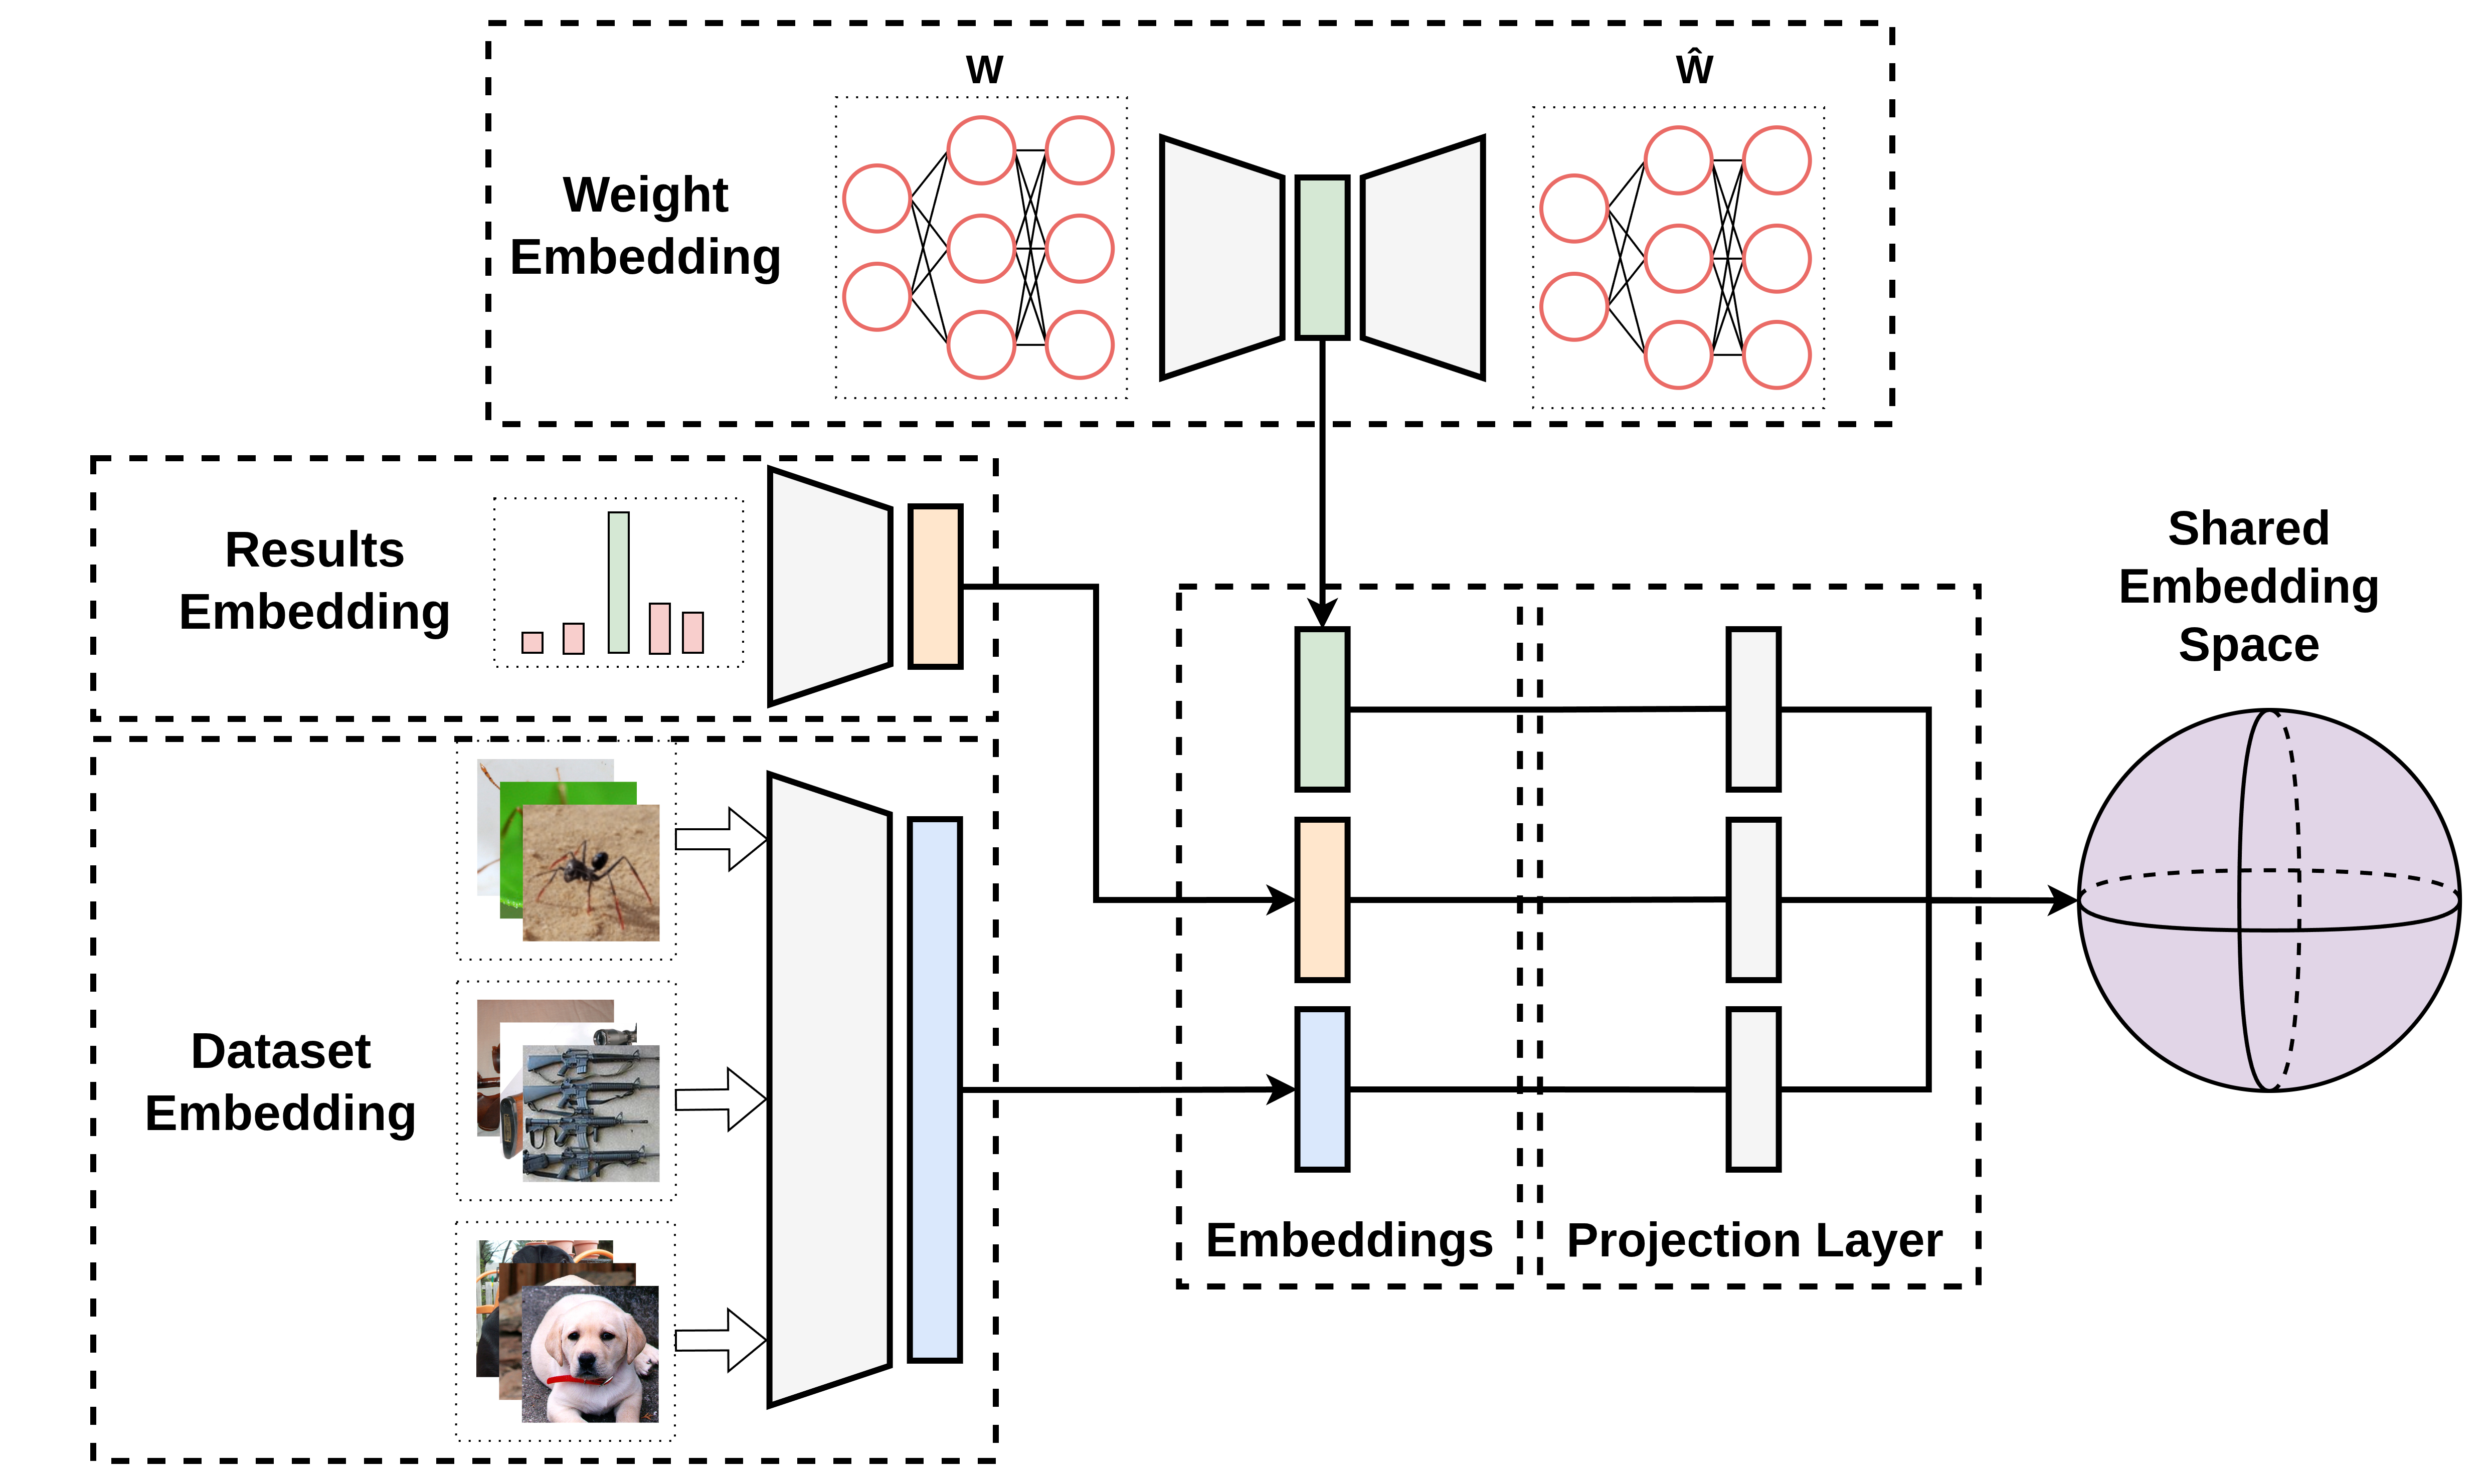
\includegraphics[width=0.75\linewidth]{pipeline.png}
    \caption[The process of embedding a dataset, model weigths and results into a shared embedding space ]{The process of embedding a dataset, model weigths and results into a shared embedding space. }
    \label{fig:pipeline_2}
\end{figure}

The problem of data generation, introduced in Section~\ref{sec:data_gen}, establishes a diverse collection of $(\mathcal{D}, \mathcal{W}, \mathcal{R})$ triplets by systematically varying datasets, and optimisation parameters. This process ensures a sufficiently rich space of weights and results for downstream learning.  

Building on this foundation, Section~\ref{sec:weight_enc} presents the design of the weight encoder and decoder, which transform the high-dimensional weight tensors ($\mathcal{W}$) into compact latent representations. These embeddings are optimised to preserve as much structural and functional information as possible while remaining computationally tractable.  

Sections~\ref{sec:data_enc} and~\ref{sec:results_enc} focus on encoding the contextual and performance information associated with each model. The dataset encoder maps each dataset ($\mathcal{D}$) into a semantic representation using pretrained CLIP features, while the results encoder transforms validation losses ($\mathcal{R}$) into fixed-size embeddings through a discretised lookup scheme. 

Finally, Section~\ref{sec:shared_enc} integrates these components within a shared latent space.The model learns to align the dataset and result embeddings with their corresponding weight representations, forming a unified space that captures the relationships between data, model parameters, and performance.

\section{Model Zoo Generation}
\label{sec:data_gen}
The construction of the Model Zoo is fundamentally driven by the need to generate a diverse, reproducible, and analytically valuable dataset of model weights for comprehensive weight-space exploration. The methodological choices detailed below ensure the resulting zoo provides sufficient statistical power and representational richness for subsequent analyses.

The foundation of the Model Zoo is the classification task, which must be both representative and computationally manageable. Given that ImageNet is an established benchmark for representation learning in computer vision, its rich feature set was recognized as the appropriate basis for defining the task. To maintain a manageable level of complexity for large-scale generation and maximize the number of unique training instances, the core problem was defined as classifying randomly selected subsets of three ImageNet classes. This decision ensures the models are trained on high-fidelity, real-world visual features while simultaneously creating a highly flexible input-data space through numerous possible permutations.

The architecture was uniformly set to the ResNet-18 backbone across the entire zoo population, with only the final fully connected layer modified to accommodate the three-class classification task. By standardizing the architecture, any observed differences in the weight-space properties are primarily attributable to the systematic variations introduced through training parameters. While initial weight-space research focused on smaller models, ResNet-18 provides a sufficient architectural challenge necessary for direct comparability against modern methods, such as the scalability demonstrated in [citepaper] over previous methods like [citepaper].

To guarantee the Model Zoo accurately reflects the diversity of the high-dimensional weight space, variation is introduced at the start of each training run. This begins with the random selection of classification classes from ImageNet, with the primary mechanism for systematic variation being the hyperparameter sampling from the distributions detailed in Table 1. Furthermore, the optimizer is randomly selected to be either Adam or Stochastic Gradient Descent (SGD). This simple choice immediately adds substantial structural diversity by forcing models to traverse fundamentally distinct optimization paths across the loss landscape.

\begin{table}[h]
    \centering
    \caption{Model Zoo Hyperparameter Sampling Distributions and Fixed Parameters}
    \begin{tabularx}{0.8\linewidth}{@{}lX@{}}
        \toprule
        Hyperparameter & Distribution / Value \\
        \midrule
        Problem Domain & Random subsets of 3 ImageNet classes \\
        Model Architecture & ResNet-18 (Fixed) \\
        Optimizer & Randomly selected: Adam or SGD \\
        Early Epoch Snapshot & Uniform, $U(5, 10)$ \\
        Maximum Epoch & Truncated Normal, $N(\mu=100, \sigma=15)$ with bounds $[50, 150]$ \\
        Learning Rate ($\eta$) & $Insert specific LR distribution$ \\
        \bottomrule
    \end{tabularx}
    \label{tbl:model_zoo_params}
\end{table}

To analyze the geometry of the weight space at different phases of optimization, two distinct weights snapshots are captured per training trajectory: an 'early epoch' checkpoint and a 'max epoch' checkpoint. The early epoch is sampled uniformly, specifically designed to capture models in low-performing, under-trained states. This intentional approach provides crucial data on the structure of the weight space's nascent landscape and the optimization trajectory. Conversely, the maximum training epoch is sampled from a truncated Normal distribution. This range ensures the model has reached a point reflective of a converged, stable local loss minimum, thereby accurately representing the typical, high-performing outcomes of model training. Finally, the total sample size, $X$, is set to the maximum number computationally feasible given resource constraints. This practical constraint ensures the generation of a statistically representative number of unique training instances necessary for robust analysis of the weight space.


% \begin{table}[!h]
%     \mytable
%     \caption{}
%     \begin{tabularx}{\linewidth}{@{}lCCCCC@{}}
%         \toprule
%         Metric     & 1 & 2 & 3 & 4 & 5 \\
%         \midrule
%         WER (\%)                        & $35.4$ & $23.5$ & $21.5$ & $21.2$ & $22.9$ \\
%         Average cluster purity (\%)       & $86.5$ & $89.7$ & $89.2$ & $88.5$ & $86.6$ \\
%         Word boundary $F$-score (\%)         & $70.6$ & $72.2$ & $71.8$ & $70.9$ & $69.4$ \\
%         Cluster2s covering 90\% of data   & 20             & 13 & 13 & 13 & 13 \\
%         \bottomrule
%     \end{tabularx}
%     \label{tbl:exemplars}
% \end{table}


% \begin{table}[!h]
%     \renewcommand{\arraystretch}{1.1}
%     \centering
%     \caption{A table with an example of using multiple columns.}
%     \begin{tabularx}{0.65\linewidth}{@{}lCCr@{}}
%         \toprule
%         & \multicolumn{2}{c}{Accuracy (\%)} \\
%         \cmidrule(lr){2-3}
%         Model    & Intermediate & Output & Bitrate\\
%         \midrule
%         Baseline & 27.5         & 26.4   & 116 \\
%         VQ-VAE   & 26.0         & 22.1   & 190 \\
%         CatVAE   & 28.7         & 24.3   & 215 \\
%         \bottomrule
%     \end{tabularx}
%     \label{tbl:abx_speaker}
% \end{table}
\newpage
\section{Weight Encoder}
\label{sec:weight_enc}
The Weight Encoder is implemented to learn a compact, functional latent representation for neural network parameters obtained from the model zoo. The objective is to train an autoencoder that encodes the parameters of each model and reconstructs them with minimal deviation from the originals. This corresponds to minimising the reconstruction loss, $\mathcal{L}_{\text{MSE}}$, as defined in Equation~\ref{eq:weight_recon_loss}. To ensure generalisation, performance is validated on a separate validation set $\mathcal{M}_{\text{val}}$, restricted to ten distinct models due to limited availability of pre-trained networks.

An intuitive baseline would be to flatten the entire ResNet18 weight matrix $\mathbf{W}_m$ into a single high-dimensional vector and train an autoencoder directly on it. However, given that ResNet18 contains over 11 million parameters, this approach is computationally infeasible and would require an impractically large dataset for the model to generalise effectively \cite{some_reference}.  

Alternative methods such as sequential tokenisation of layers (discussed in Section~\ref{sec:autoencoders}) provide a more scalable representation but introduce additional architectural complexity. Instead, we adopt a simpler yet effective two-stage compression approach, beginning with a \textit{Per-Named-Parameter PCA} transformation.  

In the first stage, dimensionality reduction is applied separately to each named parameter tensor (for example, \texttt{conv1.weight} or \texttt{fc.bias}) across all models. This preserves the modular structure of the network while tailoring the compression to the statistical properties of each parameter type. The process for determining which compression method to apply is outlined in Algorithm~\ref{alg:pca-mode-selection}.

\begin{algorithm}[H]
\caption{Mode Selection During PCA Fitting}
\label{alg:pca-mode-selection}
\begin{algorithmic}[1]
\For{each named parameter in model zoo}
    \State $V \gets \text{calculate\_variance}(\text{parameter values across all models})$
    \State $D \gets \text{calculate\_dimension}(\text{parameter values across all models})$
    \If{$V < \text{VARIANCE\_THRESHOLD}$}
        \State \text{store\_only\_mean()} \Comment{Retain only mean}
    \ElsIf{$D \leq \text{DIMENSION\_LIMIT}$}
        \State \text{store\_centered\_weights()} \Comment{Retain centered weights}
    \Else
        \State \text{fit\_IncrementalPCA()} \Comment{Fit IncrementalPCA}
    \EndIf
\EndFor
\end{algorithmic}
\end{algorithm}

Three compression modes are used:
\begin{itemize}
    \item For high-variance, high-dimensional tensors, \textit{IncrementalPCA} projects the centred weights onto a small number of principal components, retaining maximal variance in a compact coefficient representation.
    \item For small tensors (four dimensions or fewer), only centering is applied, as PCA provides negligible benefit.
    \item For low-variance tensors, only the mean value is stored, discarding coefficients entirely for maximal compression.
\end{itemize}

Following PCA, the resulting coefficient vectors obtained for each named parameter are concatenated to form a single reduced representation for each model. Each vector contains the retained PCA coefficients for one named parameter, where the number of retained components \(k_i\) varies depending on that parameter's variance structure. The concatenated coefficient vector, denoted \(\mathbf{C}_m\), thus compactly represents all named parameters of model \(m\) in a unified format. This vector is normalised using dataset-wide statistics and then serves as input to the second compression step, a deep autoencoder. This two-stage compression process is illustrated in Figure~\ref{fig:pca_ae}, showing how PCA is applied per named parameter followed by a deep autoencoder producing a compact latent representation.


\begin{figure}[!t]
    \centering
    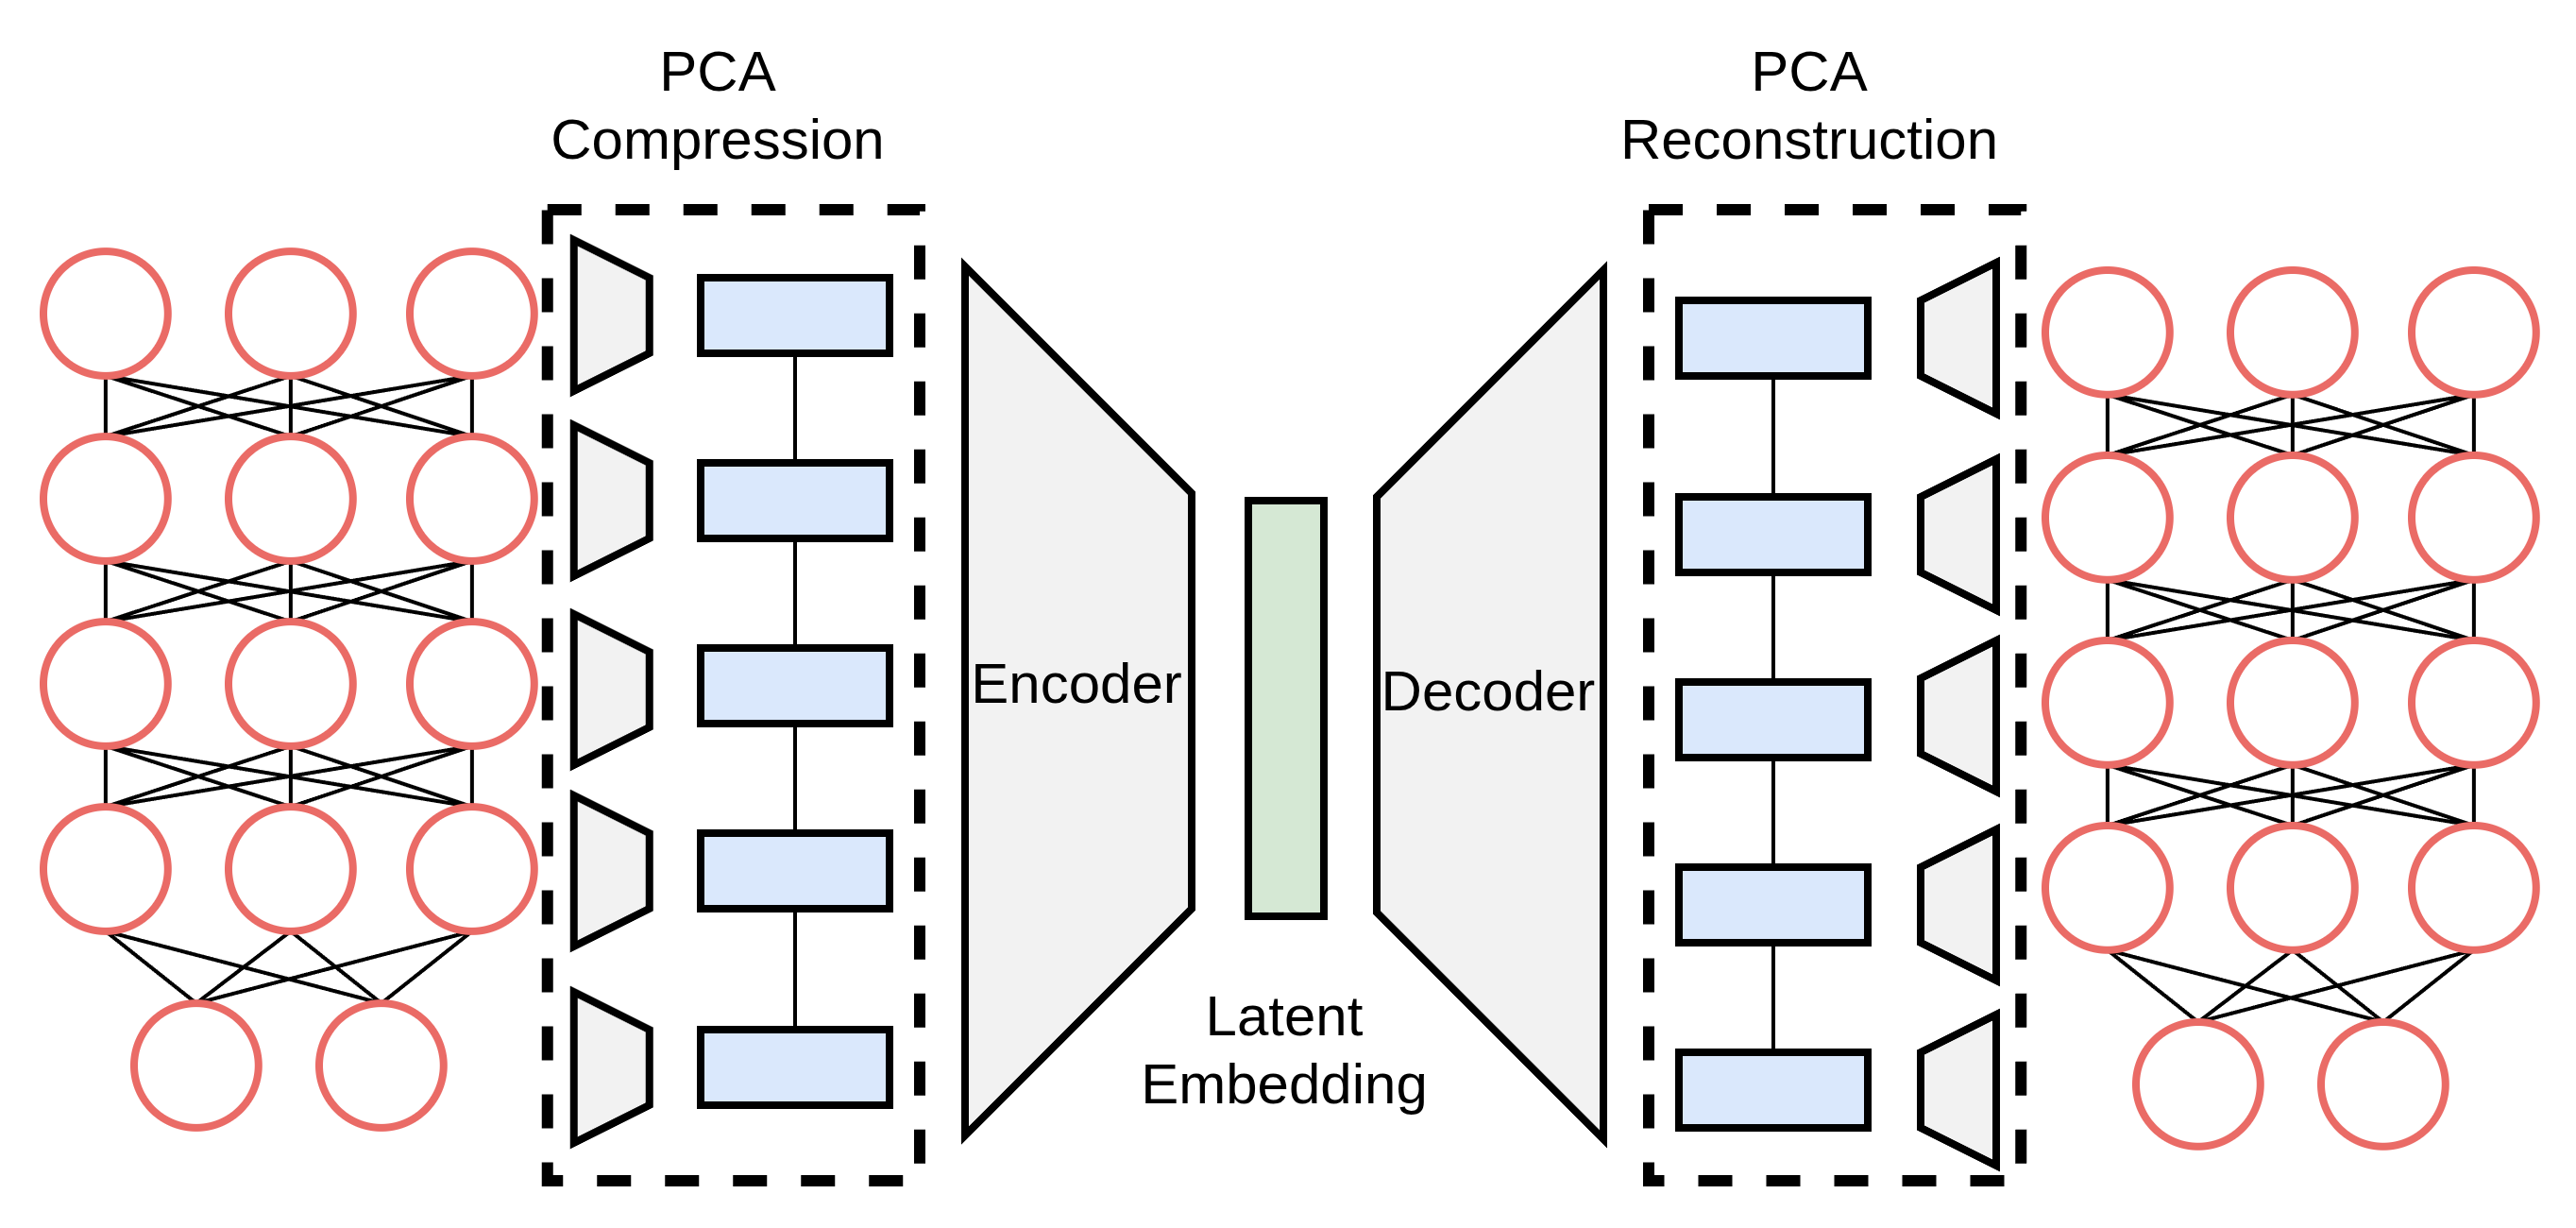
\includegraphics[width=0.75\linewidth]{pca_ae.png}
    \caption{Two-stage compression of model weights: PCA reduces each parameter tensor, followed by an autoencoder producing a compact latent representation.}

    \label{fig:pca_ae}
\end{figure}


In the second stage, the autoencoder learns a lower-dimensional latent representation of the PCA-compressed vectors. The encoder maps the normalised coefficient vector $\mathbf{C}_m$ to a compact latent representation $\mathbf{z}_m \in \mathbb{R}^{D_{\text{latent}}}$:
\[
\mathbf{z}_m = f_{\text{enc}}(\mathbf{C}_m; \theta_e),
\]
and the decoder reconstructs it as
\[
\hat{\mathbf{C}}_m = f_{\text{dec}}(\mathbf{z}_m; \theta_d).
\]
Training minimises a per-named-parameter reconstruction objective, extending the standard mean-squared error loss in Equation~\ref{eq:weight_recon_loss} to operate across all parameters:

\begin{equation}
  \mathcal{L}_{\text{AE}} = \frac{1}{|\mathcal{M}_{\text{train}}|} 
\sum_{m \in \mathcal{M}_{\text{train}}} 
\frac{1}{N_m} 
\sum_{i=1}^{N_m} 
\| \mathbf{c}_{i,m} - f_{\text{dec}}(f_{\text{enc}}(\mathbf{c}_{i,m})) \|^2_2,
  \label{eq:pca_ae_loss}
\end{equation}

where $\mathbf{c}_{i,m}$ denotes the PCA coefficient vector for the $i$-th named parameter of model $m$, and $N_m$ is the total number of named parameters for that model. This formulation ensures that the autoencoder learns to compress and reconstruct parameters in a balanced manner while maintaining structural variance across layers and modules.


After reconstruction, each parameter’s coefficients $\hat{\mathbf{c}}_{i,m}$ are transformed back into their original tensor shapes using the stored PCA statistics from the fitting stage. Specifically, for each named parameter $i$, the inverse PCA transform restores the weight tensor by reprojecting the coefficients into the original feature space and re-adding the mean vector:
\[
\hat{\mathbf{W}}_{i,m} = \mathbf{V}_i \hat{\mathbf{c}}_{i,m} + \boldsymbol{\mu}_i,
\]
where $\mathbf{V}_i$ is the PCA component matrix and $\boldsymbol{\mu}_i$ is the mean of the original parameter distribution. If PCA was not applied (for small or low-variance tensors), the stored centring or mean operations are inverted accordingly. 

The combined PCA and autoencoder encoding system offers several benefits. By applying PCA first, the dimensionality of each parameter tensor is significantly reduced, which lowers the computational and memory requirements for training the autoencoder. This high compression makes the system easier and faster to train while still capturing the dominant variance in the model weights. However, this approach also has inherent limitations. Since PCA compresses based on variance directions observed in the training models, unseen models with weights that are outliers or vary along unrepresented directions may be poorly encoded. Consequently, the system might not generalise well to models whose parameter distributions differ significantly from the training set.

\section{Dataset Encoder}
\label{sec:data_enc}

Following the discussion in Section~\ref{sec:contrastive} on contrastive learning and the CLIP framework, we adopt a pretrained CLIP visual encoder to extract semantic embeddings for the dataset classes. Each image $x$ is passed through the CLIP encoder $f_{\text{CLIP}}(\cdot)$, producing a 512-dimensional latent representation $z_x$:

\[
z_x = f_{\text{CLIP}}(x).
\]

To obtain a class-level representation, we compute the embeddings for all images belonging to a given class and average them, yielding a single 512-dimensional vector $\bar{z}_c$ that summarises the class:

\[
\bar{z}_c = \frac{1}{|X_c|} \sum_{x \in X_c} z_x,
\]

where $X_c$ denotes the set of images in class $c$. 

Finally, the embeddings for the three classes are concatenated to form the final dataset-level representation:

\[
\mathbf{z}_{\text{dataset}} = [\bar{z}_{c_1}; \bar{z}_{c_2}; \bar{z}_{c_3}] \in \mathbb{R}^{1536}.
\]

This concatenated vector serves as the input to the shared encoding stage for alignment with the weight embeddings. This approach leverages the pretrained CLIP features to provide a rich semantic summarisation of each class, ensuring that the resulting dataset representation captures meaningful visual information relevant for model alignment.

\section{Results Encoder}
\label{sec:results_enc}

To capture the performance of each model, we use the validation loss recorded at the checkpoint corresponding to the saved weights. Instead of using the raw scalar loss directly, we quantize the range of validation losses observed across the model zoo into discrete bins. Each bin is associated with a learnable 512-dimensional embedding vector, allowing the model to map a validation loss to a rich latent representation:

\[
\mathbf{r}_m = \text{Embedding}(\text{bin}(\mathcal{L}_{\text{val}, m})),
\]

where $\mathcal{L}_{\text{val}, m}$ is the validation loss of model $m$, and $\mathbf{r}_m \in \mathbb{R}^{512}$ is the corresponding learned embedding.  

This approach has several advantages. First, by representing the continuous range of validation losses with trainable embeddings, the system can learn a smooth latent space that captures nuanced performance differences between models. Second, it avoids the need to directly regress continuous loss values, which can be noisy and poorly scaled across diverse architectures or training schedules.

\section{Shared Encoding}
\label{sec:shared_enc}

The shared encoding stage aligns the dataset and results embeddings with the weight latent space. To achieve this, the dataset-level vector $\mathbf{z}_{\text{dataset}}$ from Section~\ref{sec:data_enc} and the results embedding $\mathbf{z}_{\text{results}}$ from Section~\ref{sec:results_enc} are first concatenated:

\[
\mathbf{z}_{\text{input}} = [\mathbf{z}_{\text{dataset}}; \mathbf{z}_{\text{results}}].
\]

This combined vector is then passed through a multi-layer perceptron (MLP) to produce a predicted embedding $\hat{\mathbf{z}}_{\text{weight}}$ in the weight latent space:

\[
\hat{\mathbf{z}}_{\text{weight}} = \text{MLP}(\mathbf{z}_{\text{input}}; \theta_{\text{MLP}}).
\]

Training minimises the NT-Xent contrastive loss, as described in Section~\ref{sec:contrastive} and defined in Equation~\ref{eq:multi_loss}, between $\hat{\mathbf{z}}_{\text{weight}}$ and the corresponding weight embedding $\mathbf{z}_{\text{weight}}$. Backpropagation is used to update the MLP parameters $\theta_{\text{MLP}}$:

\[
\mathcal{L}_{\text{NT-Xent}}(\hat{\mathbf{z}}_{\text{weight}}, \mathbf{z}_{\text{weight}}) \rightarrow \min_{\theta_{\text{MLP}}}.
\]

This design ensures that the mapping from dataset and results space to the weight latent space is fully differentiable and preserves the reversibility of the weight representation. Importantly, the projection is performed from dataset and results to weight space rather than the reverse: applying a non-linear transformation directly to the weight embedding would break invertibility, making it impossible to reconstruct the original weight vector from the shared representation. By contrast, pushing the dataset and results embeddings to the weight space allows the latent weight vector to remain consistent and decodable via the trained autoencoder.
% perhapsh add the hyper parameters?
